\documentclass[]{article}
\usepackage[]{graphicx}
\usepackage[]{xcolor}
\usepackage[]{adjustbox}


\begin{document}
\author{Matteo Ielacqua}
\title{Github Social}
\maketitle
    \section{Brief introduction}
    A large social network of GitHub developers which was collected from the public API in June 2019. Nodes are developers who have starred at least 10 repositories and edges are mutual follower relationships between them.
    \subsection*{Context}
    GitHub is a double scope platform: In first place is used to store and develop software , either by open source developers and by companies, secondly is a social network for developers in which them can argue about technical solution and future projects. In GitHub a user can Fork ( copy the repository in his own userspace), view the code and star a repository. The star operation is a follow operation, thus a user can track the progress on certain repository. But is also possible to follow a developer to see which project he taken part to, and that's what the network is collecting. The original scope of this network was to target each developer (node) and understand if it is a machine learning or web developer, the content of this information is available in the file musae_git_target.
    \subsection*{What to expect}
    This is a social network, so we expect a sparse graph with very few node very popular and most of them not. Most of the nodes should be part of a giant component. Triadic closure is probably given by some developers working on the same project (assumpting that the node is respecting the requirements of have starred 10 repositiories) and so we expect the presence of some big communities given by the presence of big project (like for example Unreal Engine source code or Qt company code). Sure there will a clearly manifestation of homophily, especially in those project oriented only in machine learning or webdesign, but what about bigger project that requires some exchanges of competences? The answer in obvliviously that heterophily has to be seen in those contexts. 

    \section{Basic Measures}
    
    \subsection*{Degree}
    \begin{itemize}
        \item Min: 1
        \item Max: 9458
        \item Mean: 15.3317
    \end{itemize}

    \begin{figure}[htp]
        \centering
        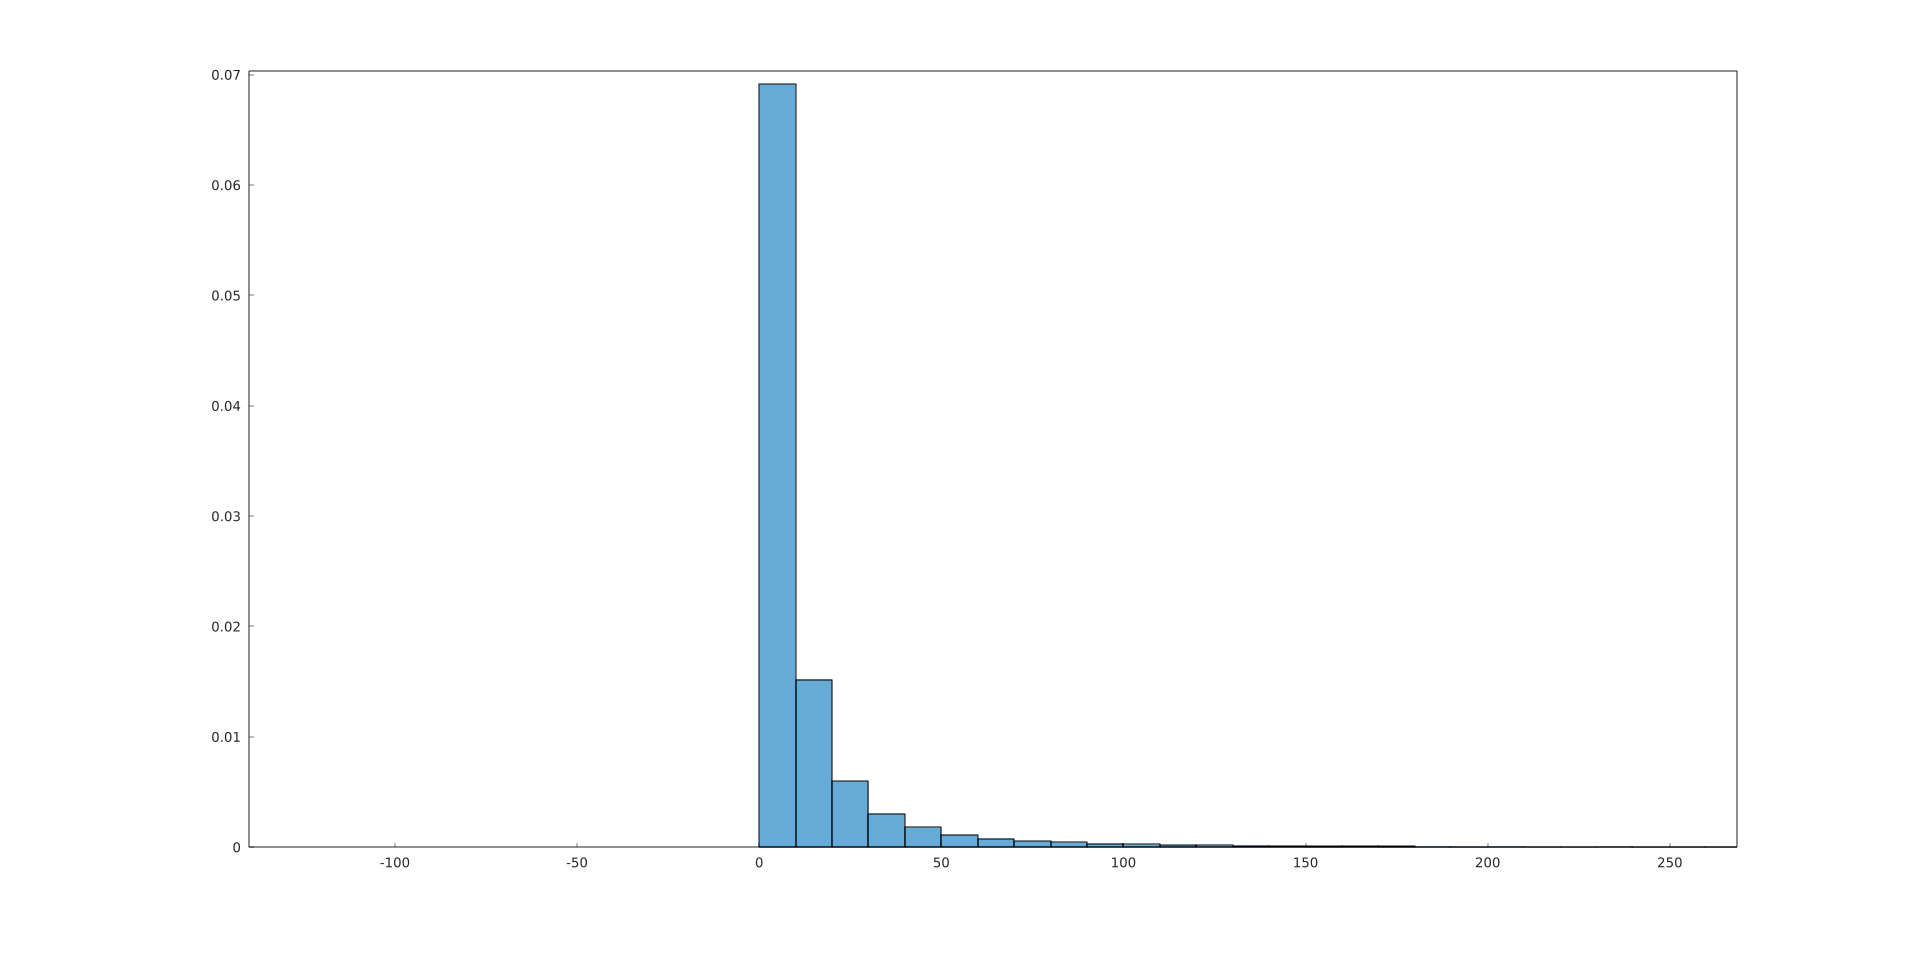
\includegraphics[scale=0.20]{./charts/degree_distribution.png}
    \end{figure}

    

\end{document}